\documentclass{article}

\usepackage{graphicx}
\usepackage{amsmath}
\usepackage{amssymb} % \gtrsim is defined here

\begin{document}
\part{Normalized clustering coefficients}


\section{Introduction}

\subsection{Current measures for clustering}

Local clustering coefficient \cite{Watts1998}:

\begin{equation}
    c_i = 
    \left\{
    	\begin{array}{ll}
    		\dfrac{2 T_i}{k_i (k_i-1)}  & \mbox{if } k_i > 1 \\
    		0 & \mbox{if } k_i \leq 1,
    	\end{array}
    \right.
\end{equation}

where $T_i$ is the number of triangles passing through vertex $i$ and $k_i$ is its degree.

Average Watts-Strogatz clustering coefficient:
\begin{equation}
    \bar{C} = \dfrac{1}{N} \sum_i c_i.
\end{equation}

Obs: This average is taken over all the nodes in the network. Some authors use, instead, the only the nodes with degree greater than 1. It is important to be aware of that when interpreting results of other authors.

Degree-dependent clustering coefficient \cite{Vazquez2002Large-scaleInternet}:

\begin{equation}
    \bar{c}(k) = \dfrac{1}{N_k} \sum_{i\in Y(k)} c_i = \dfrac{1}{k(k-1)N_k} \sum_{i\in Y(k)} 2T_i,
\end{equation}

where $N_k$ is the number of nodes with degree $k$ and $Y(k)$ is the set of such nodes.

The quantities $\bar{C}$ and $\bar{c}(k)$ are related by

\begin{equation}
    \bar{c} = \sum_k p(k) \bar{c}(k),
\end{equation}

$p(k)$ being the degree distribution.

A different global transitivity measure $C$ was introduced by Newman in \cite{Newman2003}, and is defined as 

\begin{equation}
    C = \dfrac{2T}{\sum_i k_i (k_i-1)},
\end{equation}

where $T = \sum_i T_i$ is the number of triangles in the network.

The two global clustering coefficients have similar definitions and, in fact, for some networks both have similar values. In particular, for an uncorrelated network, $\bar{C}$, $\bar{c}(k)$ and $C$ are identical and its value can be computed as \cite{NewmanBook} 

\begin{equation} \label{eq:Cunc}
C_{\mathrm{unc}} = \dfrac{1}{N} \dfrac{\left[ \langle k^2 \rangle - \langle k \rangle  \right]^2}{\langle k \rangle^3}.
\end{equation}

Nevertheless, these coefficients do differ significantly in some cases, as can be seen in \cite{Bollobs2004, Estrada2011}.

\subsection{Normalized clustering coefficient}

We define the normalized clustering coefficients

\begin{equation} \label{eq:Cnorm}
C_{\mathrm{norm}} = \dfrac{C - C_{\mathrm{rand}}}{C_{\mathrm{max}} - C_{\mathrm{rand}}}\qquad \text{and} \qquad
\bar{c}_{\mathrm{norm}} = \dfrac{\bar{c} - \bar{c}_{\mathrm{rand}}}{\bar{c}_{\mathrm{max}} - \bar{c}_{\mathrm{rand}}}
\end{equation}

$C_{\mathrm{rand}}$ and $\bar{c}_{\mathrm{rand}}$ represent the average of the clustering coefficient computed for an ensemble of random networks with the same degree sequence as the original network, and $C_{\mathrm{max}}$ and $\bar{c}_{\mathrm{max}}$ correspond to the maximum clustering values that can be achieved over the networks in the ensemble. In our work, we will consider the ensamble of all networks having the same degree sequence as the original network.

There are differen posibilities in which $C_{\mathrm{rand}}$ can be defined. One way is using the expected value for an uncorrelated network, given by Equation \ref{eq:Cunc}, which can be easily computing from the degree sequence. Unfortunately, this measure has some problems for heterogeneous graphs (for which the hypothesis of no degree-degree correlations is not satisfied), as is exemplified in Appendix \ref{app:Cunc}. The alternative is to create instances of randomized versions of the network and define $C_{\mathrm{rand}}$ as the average of the clustering coefficient for a set of such instances. In this line, we used two different randomization procedures. The first one is the Configuration Model \cite{Molloy1995ASequence}, and the second method consists in randomizing the original network by degree-preserving edge rewiring. %The two randomization approaches are similar, but not exactly the same. One of the main differences is that when the network is dense ($\langle k \rangle \gtrsim 10$)

The Configuration Model is an algorithm that allows to build a network with a given degree sequence from scratch. It works as follows. We start with an empty graph with $N$ nodes (being $N$ the size of the desired network). We then attach to each node a number of ``half-edges'' or stubs equal to the node's degree. Then, with uniform probability we pick a pair of stubs and join them, forming an edge. We repeat this step until there is no more free stubs. The algorithm does not impose any restriction on the graph connectivity, and can even create double-edges and self-loops. If one is interested in generating simple graphs, there are two options. The first is to repeatedly apply the algorithm until the resulting graph is simple. It has been proved [TODO: add reference] that by doing that, the sampling is uniform among all the simple graph with the given degree sequence. The downside of this alternative is that it can be computationally prohibitive, in particular for networks with diverging $\langle k^2 \rangle$, where the probability sampling a simple graph is very low \cite{NewmanBook}. The second alternative is to remove all the self-loops and double-edges from the sampled graph. The expected number of such edges is $\frac{1}{2} \left[ (\langle k^2 \rangle - \langle k \rangle ) / \langle k \rangle \right]^2$ \cite{NewmanBook}, so it vanishes for $N\rightarrow \infty$ as long as $\langle k^2 \rangle$ remains bounded. This means that this second alternative is practical for networks that are not too heterogeneous. In this work, we chose this second alternative, for which we created 100 random graphs and then took the average of the corresponding clustering coefficients.

The method of degree-preserving edge rewiring (also known as edge swapping or markov chain approach) has been widely used in the literature \cite{Orsini2015QuantifyingNetworks} [TODO: add more references]. It consists on randomly selecting a pair of non-adjacent edges and, if no double edge is created in the process, swapping them. This procedure preserves the degree sequence, but destroys degree correlations. It has been shown that a number $\gtrsim M$ of swaps is enough to decorrelate the network. Here, we performed 10 independent realizations with a total of $n = 100 M$ swaps for networks small networks ($M < 100000$) and  $n = 10 M$ swaps for big networks ($M < 100000$) [TODO: add references related to mixing time and ergodicity for edge swapping]. 

\subsection{Maximum clustering coefficient}

The definitions given by equation \ref{eq:Cnorm} require the knowledge of the greatest value for the clustering coefficient that can be achieved by a graph having a specified degree sequence. In this section we will address how to compute that value.

\subsubsection{Approximation of $C_{\mathrm{max}}$}

{\bf Havel-Hakimi algorithm:}

This is a known algorithm that is very useful because it allows to determine whether a given degree sequence is graphic or not \cite{Hakimi1962}. It is based on the Havel-Hakimi theorem, which states that the degree sequence $S = [k_1, k_2, ..., k_N]$, where $k_i \geq k_j,\; \forall i\leq j$, is graphic if and only if the sequence $S' = [k_2-1, k_3-1, ..., k_{k_1+1}-1, k_{k_1+2} ,..., k_N]$ is also graphic. If the given list $S$ is graphic, then the theorem will be applied at most $N-1$ times setting in each further step $S:=S'$. Note that it can be necessary to sort this list again. This process ends when the whole list $S'$ consists of zeros. In each step of the algorithm one constructs the edges of a graph with vertices $v_1, ..., v_N$, i.e. if it is possible to reduce the list $S$ to $S'$, then we add edges $\lbrace v_1, v_2 \rbrace, \lbrace v_1, v_3 \rbrace, \lbrace v_1, v_{d_1+1} \rbrace,$. When the list $S$ cannot be reduced to a list $S'$ of non-negative integers in any step of this approach, the theorem proves that the list $S$ from the beginning is not graphic.

The advantage of this algorithm is that it always converges when the original sequence is graphic and that the resulting graph es quite clusterized. The disadvantage is that in general it doesn't give the most clusterized graph. For example, given the degree sequence $S_1 = [3, 3, 2, 2, 2, 1, 1]$, the result of the algorithm is the graph in left side of figure \ref{fig:graph_3322211}, whilst the most clustered graph for that degree sequence is the graph in the right part of the figure.

\begin{figure}[h!]
\centering
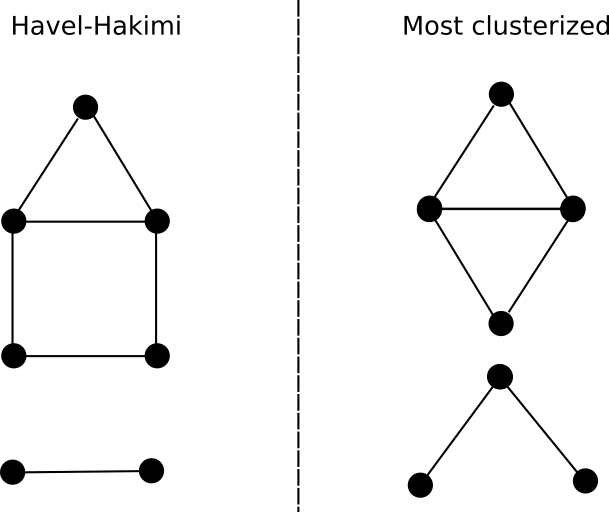
\includegraphics[scale=0.8]{./figs/graph_3322211.png}
\caption{Graphs obtained from the degree sequence $S_1 = [3, 3, 2, 2, 2, 1, 1]$}
\label{fig:graph_3322211}
\end{figure}

{\bf Greedy algorithm:}

This algorithm is similar as the Havel-Hakimi algorithm, with the difference that at each step the list is not sorted. This algorithm gives very good results for most of the real-world networks we studied (the resulting graph is more clusterized than the graph using the Havel-Hakimi algorithm). In particular, in the example in figure \ref{fig:graph_3322211}, it finds the most clusterized graph. Also, comparing with Monte Carlo simulations, it seems that this algorithm finds graphs with a clustering coefficient very close to the maximum. 

The main disadvantage of this algorithm is that it doesn't always converge. One counterexample is the degree sequence $S_2 = [3, 3, 2, 2, 2, 2]$. After adding the edges $\lbrace v_1, v_2 \rbrace, \lbrace v_1, v_3 \rbrace, \lbrace v_1, v_4 \rbrace, \lbrace v_2, v_3 \rbrace, \lbrace v_2, v_4 \rbrace, \lbrace v_5, v_6 \rbrace$, the algorithm is stuck, as there is no possible pair of nodes where to put the last edge. To overcome this flaw, we  perform the following modification. Whenever the algorithm get stuck, lets say after adding the edge $\lbrace v_i, v_j \rbrace$, we remove this edge and try to connect node $v_i$ with $v_{j+1}$. If the algorithm stuck after adding the edge $\lbrace v_i, v_N \rbrace$, we try with $\lbrace v_{i+1}, v_j \rbrace$. This way, the algorithm always converges. 

In most cases, this algorithm seems to converge to graphs very close to the most clustered graph. But if we see the example $S_2$, we can show that the result of the algorithm is the graph in the right side of figure.

\begin{figure}[h!]
\centering
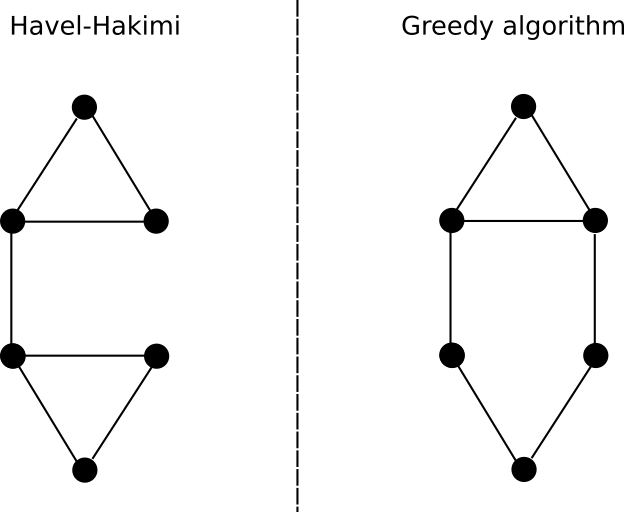
\includegraphics[scale=0.8]{./figs/graph_332222.png}
\caption{Graphs obtained from the degree sequence $S_1 = [3, 3, 2, 2, 2, 2]$}
\label{fig:graph_332222}
\end{figure}


\appendix
\section{Problems with $C_{\mathrm{unc}}$} \label{app:Cunc}

Equation \ref{eq:Cunc} is valid under the condition that no degree-degree correlation exist. In graphs with an heterogeneous degree distribution, such correlations are unavoidable, and this expresion could give incorrect values. Lets consider a few examples. 

Suppose we have a star graph with $N+1$ nodes. This graph has one single node with degree $N$ and $N$ nodes with degree $1$. the first and second momenta of the degree distribution are 

\begin{align}
    \langle k \rangle &= \dfrac{1}{N+1} \sum_{i=0}^N k_i = \dfrac{1\times N + N \times 1}{N+1} = \dfrac{2N}{N+1} \nonumber \\
    \langle k^2 \rangle &= \dfrac{1}{N+1} \sum_{i=0}^N k_i^2 = \dfrac{1\times N^2 + N \times 1^2}{N+1} = \dfrac{N^2 + N}{N+1} = N
\end{align}

If we apply equation \ref{eq:Cunc} to this particular case, we obtain

\begin{equation}
    C_{\mathrm{unc}} = \dfrac{1}{N+1}\dfrac{\left(N^2-\dfrac{2N}{N+1} \right)^2}{\left(\dfrac{2N}{N+1} \right)^3}= \dfrac{\left[N^2(N+1)-2N\right]^2}{(2N)^3} = \dfrac{(N^3+N^2-2N)^2}{8N^3},
\end{equation}

which is an increasing function of $N$ and is greater than 1 for $N \geq 3$.
\\

Now suppose we have a sparse network (with mean degree independent of $N$) and with degree distribution with second momentum scaling as $\langle k^2 \rangle \sim N^{\alpha}$, with $\alpha > 0$. In this case, equation \ref{eq:Cunc} gives

\begin{equation}
    C_{\mathrm{unc}} \sim N^{2\alpha},
\end{equation}

which is unbounded for $\alpha > 0$. That means that the expression for the expected clustering coefficient in uncorrelated networks is not valid for networks that are too heterogeneous. 

Now, lets consider the case in which we have a very connected hub with degree $k_{\mathrm{max}} \sim N^{\alpha}$. Suppose also that the degree of the rest of the nodes doesn't scale with $N$. In this case, we have, for $N\gg 1$, 

\begin{align}
    \langle k \rangle &\sim N^{\alpha - 1} \nonumber \\
    \langle k^2 \rangle &\sim N^{2\alpha-1} \nonumber 
\end{align}

Then, equation \ref{eq:Cunc} gives 

\begin{equation}
    C_{\mathrm{unc}} \sim \dfrac{1}{N} \dfrac{(N^{2\alpha-1} - N^{\alpha - 1})^2}{N^{3(\alpha - 1})} \sim \dfrac{N^{4\alpha-2}}{N^{3\alpha-2}} \sim N^{\alpha}.
\end{equation}

Thus, if the hub scales with $N$ with any positive exponent, the expected clustering coefficient diverges.


\bibliographystyle{ieeetr}
\bibliography{more_references}

\end{document}